\documentclass[11pt,]{article}
\usepackage{lmodern}
\usepackage{amssymb,amsmath}
\usepackage{ifxetex,ifluatex}
\usepackage{fixltx2e} % provides \textsubscript
\ifnum 0\ifxetex 1\fi\ifluatex 1\fi=0 % if pdftex
  \usepackage[T1]{fontenc}
  \usepackage[utf8]{inputenc}
\else % if luatex or xelatex
  \ifxetex
    \usepackage{mathspec}
  \else
    \usepackage{fontspec}
  \fi
  \defaultfontfeatures{Ligatures=TeX,Scale=MatchLowercase}
\fi
% use upquote if available, for straight quotes in verbatim environments
\IfFileExists{upquote.sty}{\usepackage{upquote}}{}
% use microtype if available
\IfFileExists{microtype.sty}{%
\usepackage{microtype}
\UseMicrotypeSet[protrusion]{basicmath} % disable protrusion for tt fonts
}{}
\usepackage[margin=1.0in]{geometry}
\usepackage{hyperref}
\hypersetup{unicode=true,
            pdftitle={Who are ASM Journals? A Gender-based Analysis},
            pdfborder={0 0 0},
            breaklinks=true}
\urlstyle{same}  % don't use monospace font for urls
\usepackage{graphicx,grffile}
\makeatletter
\def\maxwidth{\ifdim\Gin@nat@width>\linewidth\linewidth\else\Gin@nat@width\fi}
\def\maxheight{\ifdim\Gin@nat@height>\textheight\textheight\else\Gin@nat@height\fi}
\makeatother
% Scale images if necessary, so that they will not overflow the page
% margins by default, and it is still possible to overwrite the defaults
% using explicit options in \includegraphics[width, height, ...]{}
\setkeys{Gin}{width=\maxwidth,height=\maxheight,keepaspectratio}
\IfFileExists{parskip.sty}{%
\usepackage{parskip}
}{% else
\setlength{\parindent}{0pt}
\setlength{\parskip}{6pt plus 2pt minus 1pt}
}
\setlength{\emergencystretch}{3em}  % prevent overfull lines
\providecommand{\tightlist}{%
  \setlength{\itemsep}{0pt}\setlength{\parskip}{0pt}}
\setcounter{secnumdepth}{0}
% Redefines (sub)paragraphs to behave more like sections
\ifx\paragraph\undefined\else
\let\oldparagraph\paragraph
\renewcommand{\paragraph}[1]{\oldparagraph{#1}\mbox{}}
\fi
\ifx\subparagraph\undefined\else
\let\oldsubparagraph\subparagraph
\renewcommand{\subparagraph}[1]{\oldsubparagraph{#1}\mbox{}}
\fi

%%% Use protect on footnotes to avoid problems with footnotes in titles
\let\rmarkdownfootnote\footnote%
\def\footnote{\protect\rmarkdownfootnote}

%%% Change title format to be more compact
\usepackage{titling}

% Create subtitle command for use in maketitle
\newcommand{\subtitle}[1]{
  \posttitle{
    \begin{center}\large#1\end{center}
    }
}

\setlength{\droptitle}{-2em}

  \title{\textbf{Who are ASM Journals? A Gender-based Analysis}}
    \pretitle{\vspace{\droptitle}\centering\huge}
  \posttitle{\par}
    \author{}
    \preauthor{}\postauthor{}
    \date{}
    \predate{}\postdate{}
  
\usepackage{booktabs}
\usepackage{longtable}
\usepackage{array}
\usepackage{multirow}
\usepackage[table]{xcolor}
\usepackage{wrapfig}
\usepackage{float}
\usepackage{colortbl}
\usepackage{pdflscape}
\usepackage{tabu}
\usepackage{threeparttable}
\usepackage{threeparttablex}
\usepackage[normalem]{ulem}
\usepackage{makecell}
\usepackage{caption}

\usepackage{helvet} % Helvetica font
\renewcommand*\familydefault{\sfdefault} % Use the sans serif version of the font
\usepackage[T1]{fontenc}

\usepackage[none]{hyphenat}

\usepackage{setspace}
\doublespacing
\setlength{\parskip}{1em}

\usepackage{lineno}

\usepackage{pdfpages}
\floatplacement{figure}{H} % Keep the figure up top of the page
\usepackage{booktabs}
\usepackage{longtable}
\usepackage{array}
\usepackage{multirow}
\usepackage{wrapfig}
\usepackage{float}
\usepackage{colortbl}
\usepackage{pdflscape}
\usepackage{tabu}
\usepackage{threeparttable}
\usepackage{threeparttablex}
\usepackage[normalem]{ulem}
\usepackage{makecell}
\usepackage{xcolor}

\begin{document}
\maketitle

\begin{verbatim}
## [1] "reviewer_data"
\end{verbatim}

\begin{verbatim}
## [1] "sub_first_auth"
## [1] "sub_corres_auth"
\end{verbatim}

\begin{verbatim}
## [1] "pot_rev_data"
\end{verbatim}

\begin{verbatim}
## [1] "sub_mid_auth"
## [1] "sub_last_auth"
\end{verbatim}

\vspace{35mm}

Running title: A gender-based analysis of ASM journals

\vspace{35mm}

Ada K. Hagan\({^1}\), Begüm D. Topçuoğlu\({^1}\), Hazel Barton\({^2}\),
Patrick D. Schloss\textsuperscript{1\(\dagger\)}

\vspace{40mm}

\(\dagger\) To whom correspondence should be addressed:
\href{mailto:pschloss@umich.edu}{\nolinkurl{pschloss@umich.edu}}

1. Department of Microbiology and Immunology, University of Michigan,
Ann Arbor, MI 48109

2. Department of Biology, University of Akron, Akron, OH

\newpage

\linenumbers

\subsection{Abstract}\label{abstract}

\subsection{Importance}\label{importance}

\subsection{Introduction}\label{introduction}

Evidence has accumulated over the decades that academic research has a
representation problem. While at least 50\% of biology Ph.D.~graduates
are women, the number of women in postdoctoral positions and
tenure-track positions are less than 40 and 30\%, respectively
@article\{sheltzer\_elife\_2014\}. Studies examining other metrics such
as race and ethnicity find that less than 10\% of all science and
engineering doctorates were awarded to underrepresented minorities,
while less than 25\% of science and engineering doctorates in early
career academia identify as non-white (NSF ADVANCE, 2014). Predictabily,
the disparities increase alongside academic rank
@article\{potvin\_diversity\_2018\}. There have been many proposed
reasons for these disparities (particularly against women) that include
biases in training and hiring, the impact of children on career
trajectories, a lack of support for primary caregivers, a lack of
recognition, and less productivity as measured by research publications.
\textbf{Add citations} These issues do not act independant of each
other, instead they are cumulative over time for both individuals and
the community. Accordingly, addressing these issues necessitates
multi-level approaches from all insititutions and members of the
scientific community.

Recently, scientific societies and publishers have begun examining
internal submissions data to evaluate representation of, and bias
against, women in their peer review processes. The American Geological
Union found that while the acceptance rate of women-authored
publications was greater than that for publications authored by men,
women submitted fewer manuscripts than men and were used as reviewers
only 20\% of the time (Lerback, 2017), a factor influenced by the gender
of the editor (Fox, 2016). Despite the disproportional representation of
lead women authors, several studies have concluded that there is no
significant bias aginst papers authored by women (C\&W, 2011; Fox, 2016;
Handly, 2015; Edwards, 2018). Conversely, two recent studies---one of
the peer review process at eLife, a broad scope biology journal, and the
other of outcomes at six ecology and evolution journals---found that
women-authored papers are less likely to have positive reviews and
outcomes (Murray, 2018; Fox and Paine, 2019).

However, representation and attitudes differ by scientific field and no
studies to-date seem to have investigated academic publishing in the
field of microbiology. The American Society for Microbiology (ASM) is
one of the largest life science societies, with an average membership of
41,000 since 1990. In its mission statement, the ASM notes that it is
``an inclusive organization, engaging with and responding to the needs
of its diverse constituencies'' and pledges to ``address all members'
needs through development and assessment of programs and services.'' One
of these services is the publication of microbiology research through a
suite of 13 journals. The goal of this research study is to describe the
representation of authors, reviewers, and editors at ASM journals by
gender and associated peer review outcomes.

\subsection{Results}\label{results}

The term gatekeepers collectively refers to those that facilitate the
peer review process, such as editors-in-chief (EIC), editors, and
reviewers. Between January 2012 and August 2018, ASM published 15
different journals: \emph{Antimicrobial Agenst and Chemotherapy} (AAC),
\emph{Applied and Environmental Microbiology} (AEM), \emph{Clinical and
Vaccine Immunology} (CVI), \emph{Clinical Microbiology Reviews} (CMR),
\emph{Eukaryotic Cell} (EC), \emph{Infection and Immunity} (IAI),
\emph{Journal of Bacteriology} (JB), \emph{Journal of Clinical
Microbiology} (JCM), \emph{Journal of Virology} (JV), \emph{mBio},
\emph{Microbiology and Molecular Biology Reviews} (MMBR), \emph{Genome
Announcements} (GA, now \emph{Microbiology Resource Annoucements}),
\emph{Molecular and Cellular Biology} (MCB), \emph{mSphere} and
\emph{mSystems}. This study only examines original research manuscripts,
which eliminates three journals from the remaining analyses (CMR, GA,
and MMBR). Given the relatively small number of editors at ASM journals,
their presenting genders where identified by hand while the genders of
reviewers and authors were predicted from their first names. Assigning
gender by first name resulted in 3 possible outcomes: men, women, and
unknown (when gender could not be assigned with confidence, see Methods
for validation). + describe \# of manuscripts and authors + descriptive
study of a population -- no stats

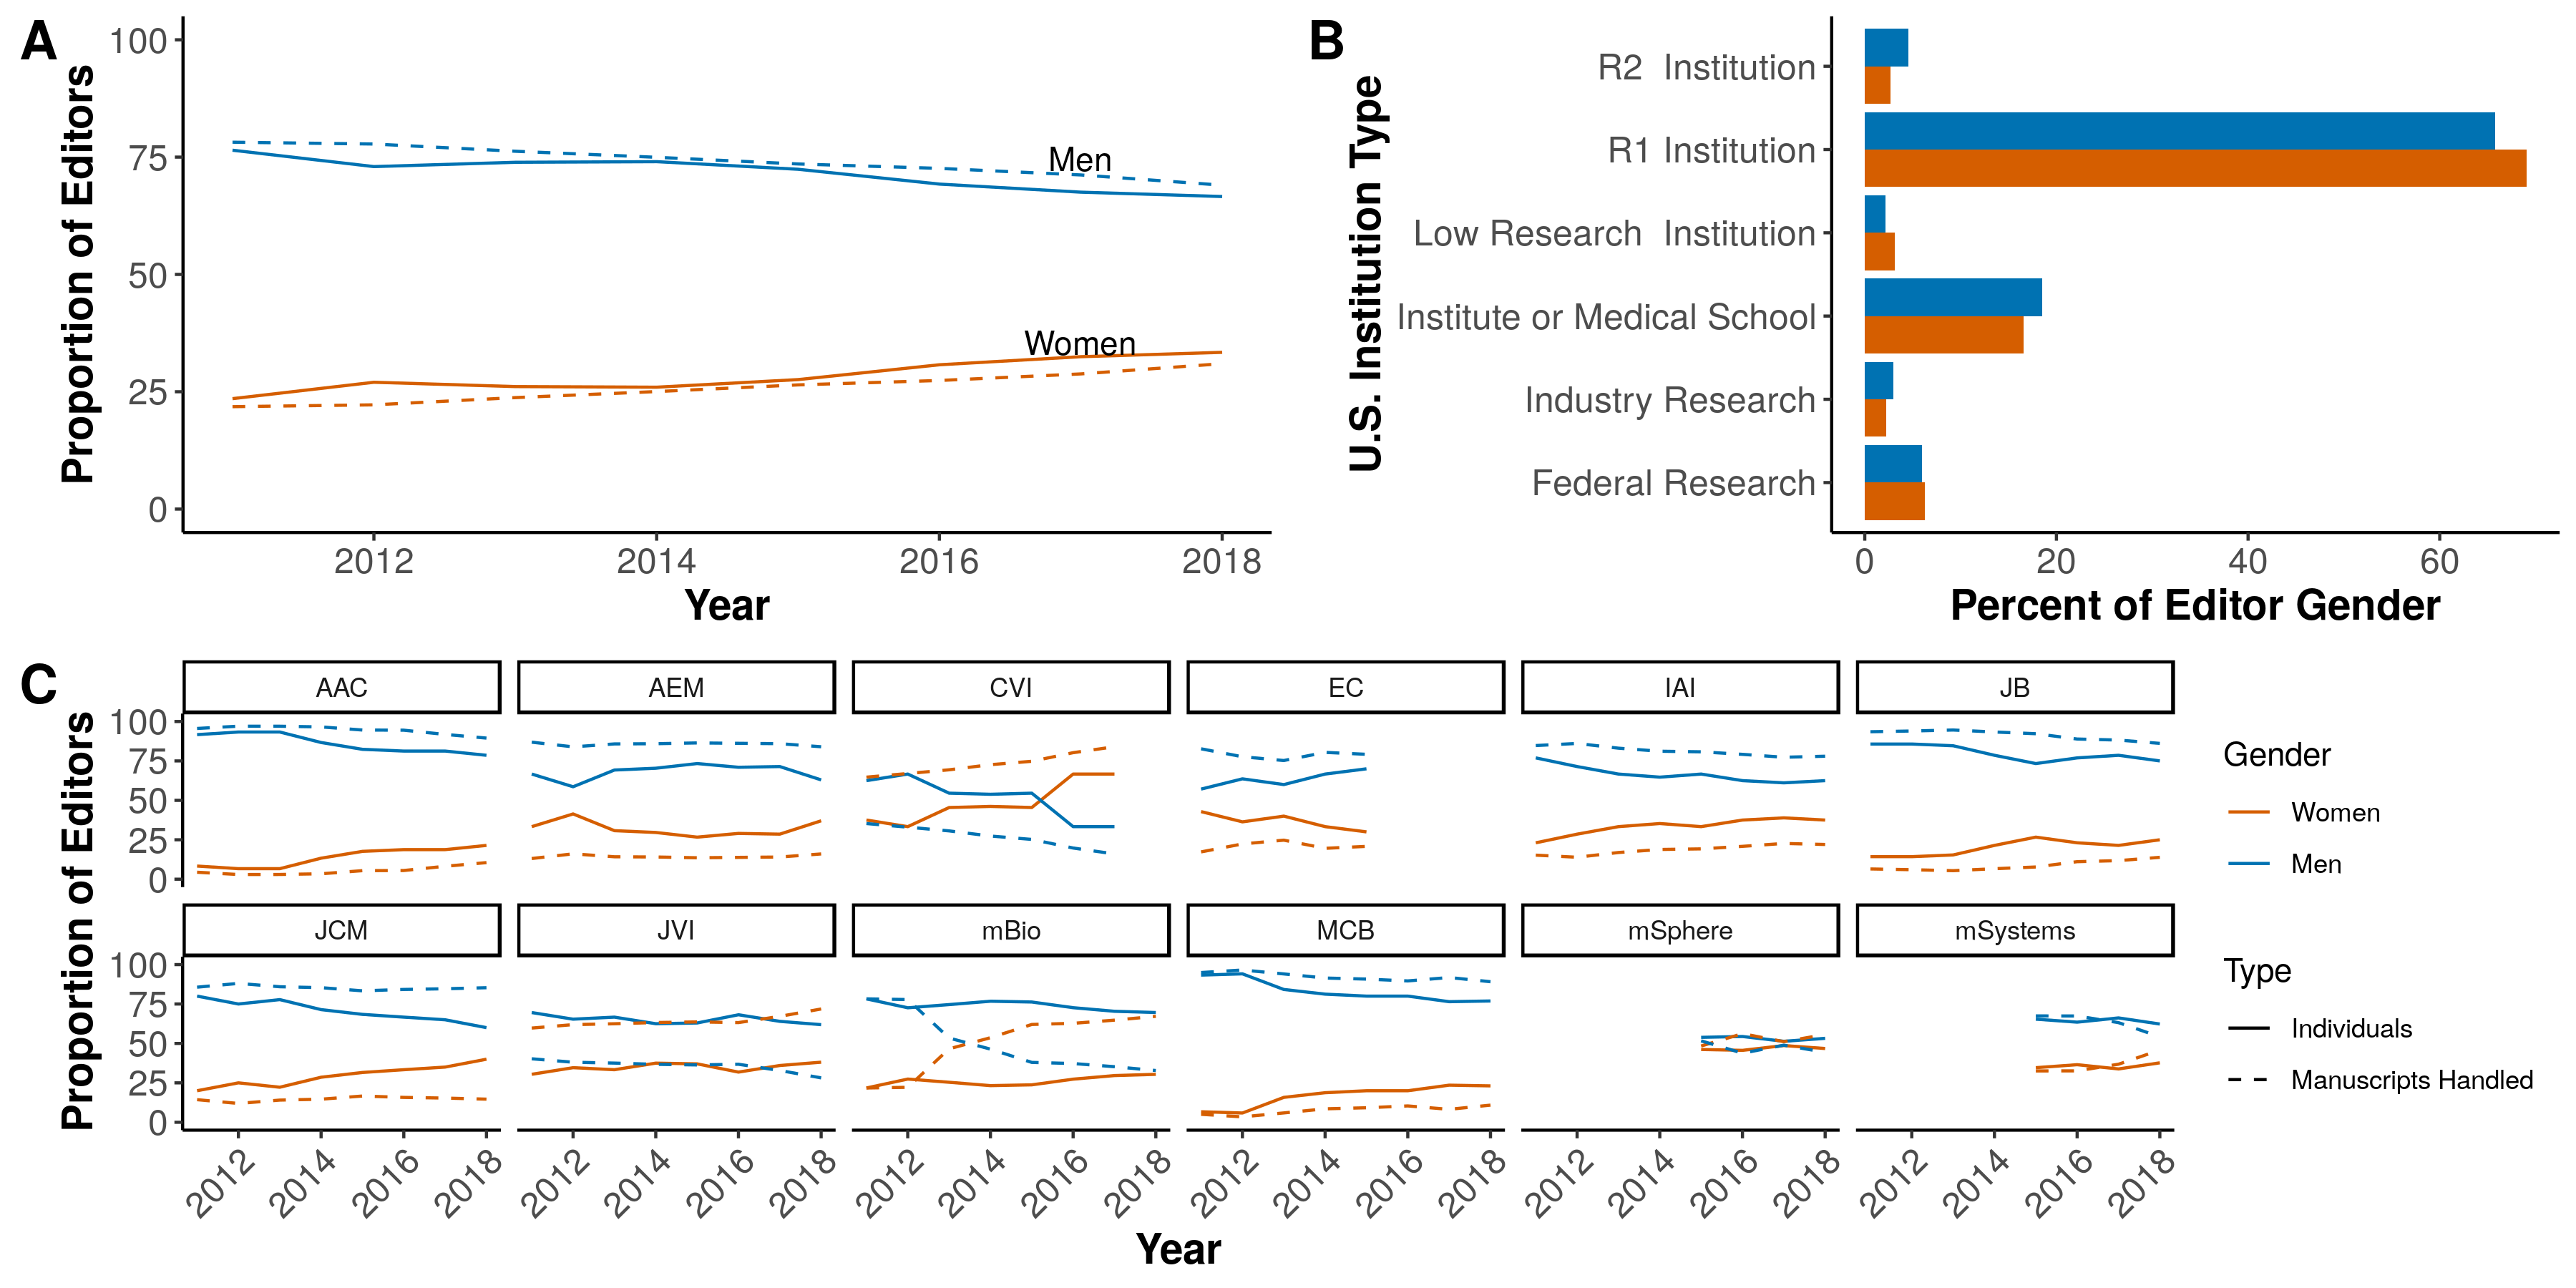
\includegraphics{Figure_1.png} \textbf{Figure 1. Gendered representation
among gatekeepers.} Proportion of editors from (A) insitution types and
(B) over time from 2012 to 2018. Editors and senior editors are pooled
together. Proportion of reviewers from (C) institution types and (D)
over time from 2012 to 2018. Each individual was counted once per
calendar year.

\textbf{Men dominate as gatekeepers and senior authors.} Each journal is
led by an editor-in-chief who manages journal scope and quality
standards. Two journals, EC and CVI were retired during the period under
study. In total, there were 17 EICs, 17.65\% of which were women. In
2013, the leadership of CVI transferred from a man EIC, to a woman. The
\emph{Journal of Virology} (JVI) has had the same woman as EIC since
2012. The EICs manage a board of editors with field expertise to help
manage the peer review process as needed. The total number of editors
over the duration of our study (senior editors and editors pooled) was
1016 and 28.74\% were women.

Over 40\% of both men and women editors are from US-based R1
institutions, with non-US and uncategorized US institutions supplying
the next largest proportions of editors (Fig. 1A). Since the start of
our study, there has been a slow trend toward gender parity of editors
(Fig. 1B). The trends for each journal studied vary considerably, though
most have slow trends toward parity (Fig. S1). CVI and \emph{mSphere}
are the only ASM journals to have accomplished equivalent representation
of both genders, with CVI having a greater proportion of women editors
than men before it was retired. EC is the only journal with an
increasing parity gap.

Our dataset contained 30704 reviewers, 24.61\% of which were women. As
with editors, the greatest proportion of reviewers (about 50\% of both
men and women) come from non-US institutions, while R1 institutions
supply the next largest cohort of reviewers (Fig. 1C). Over the time
period studied, the proportions of each gender have held steady among
reviewers at ASM journals (Fig. 1D) and is representative of both
reviewer proportions at each journal, and the potential reviewers at all
journals combined (Fig. S2).

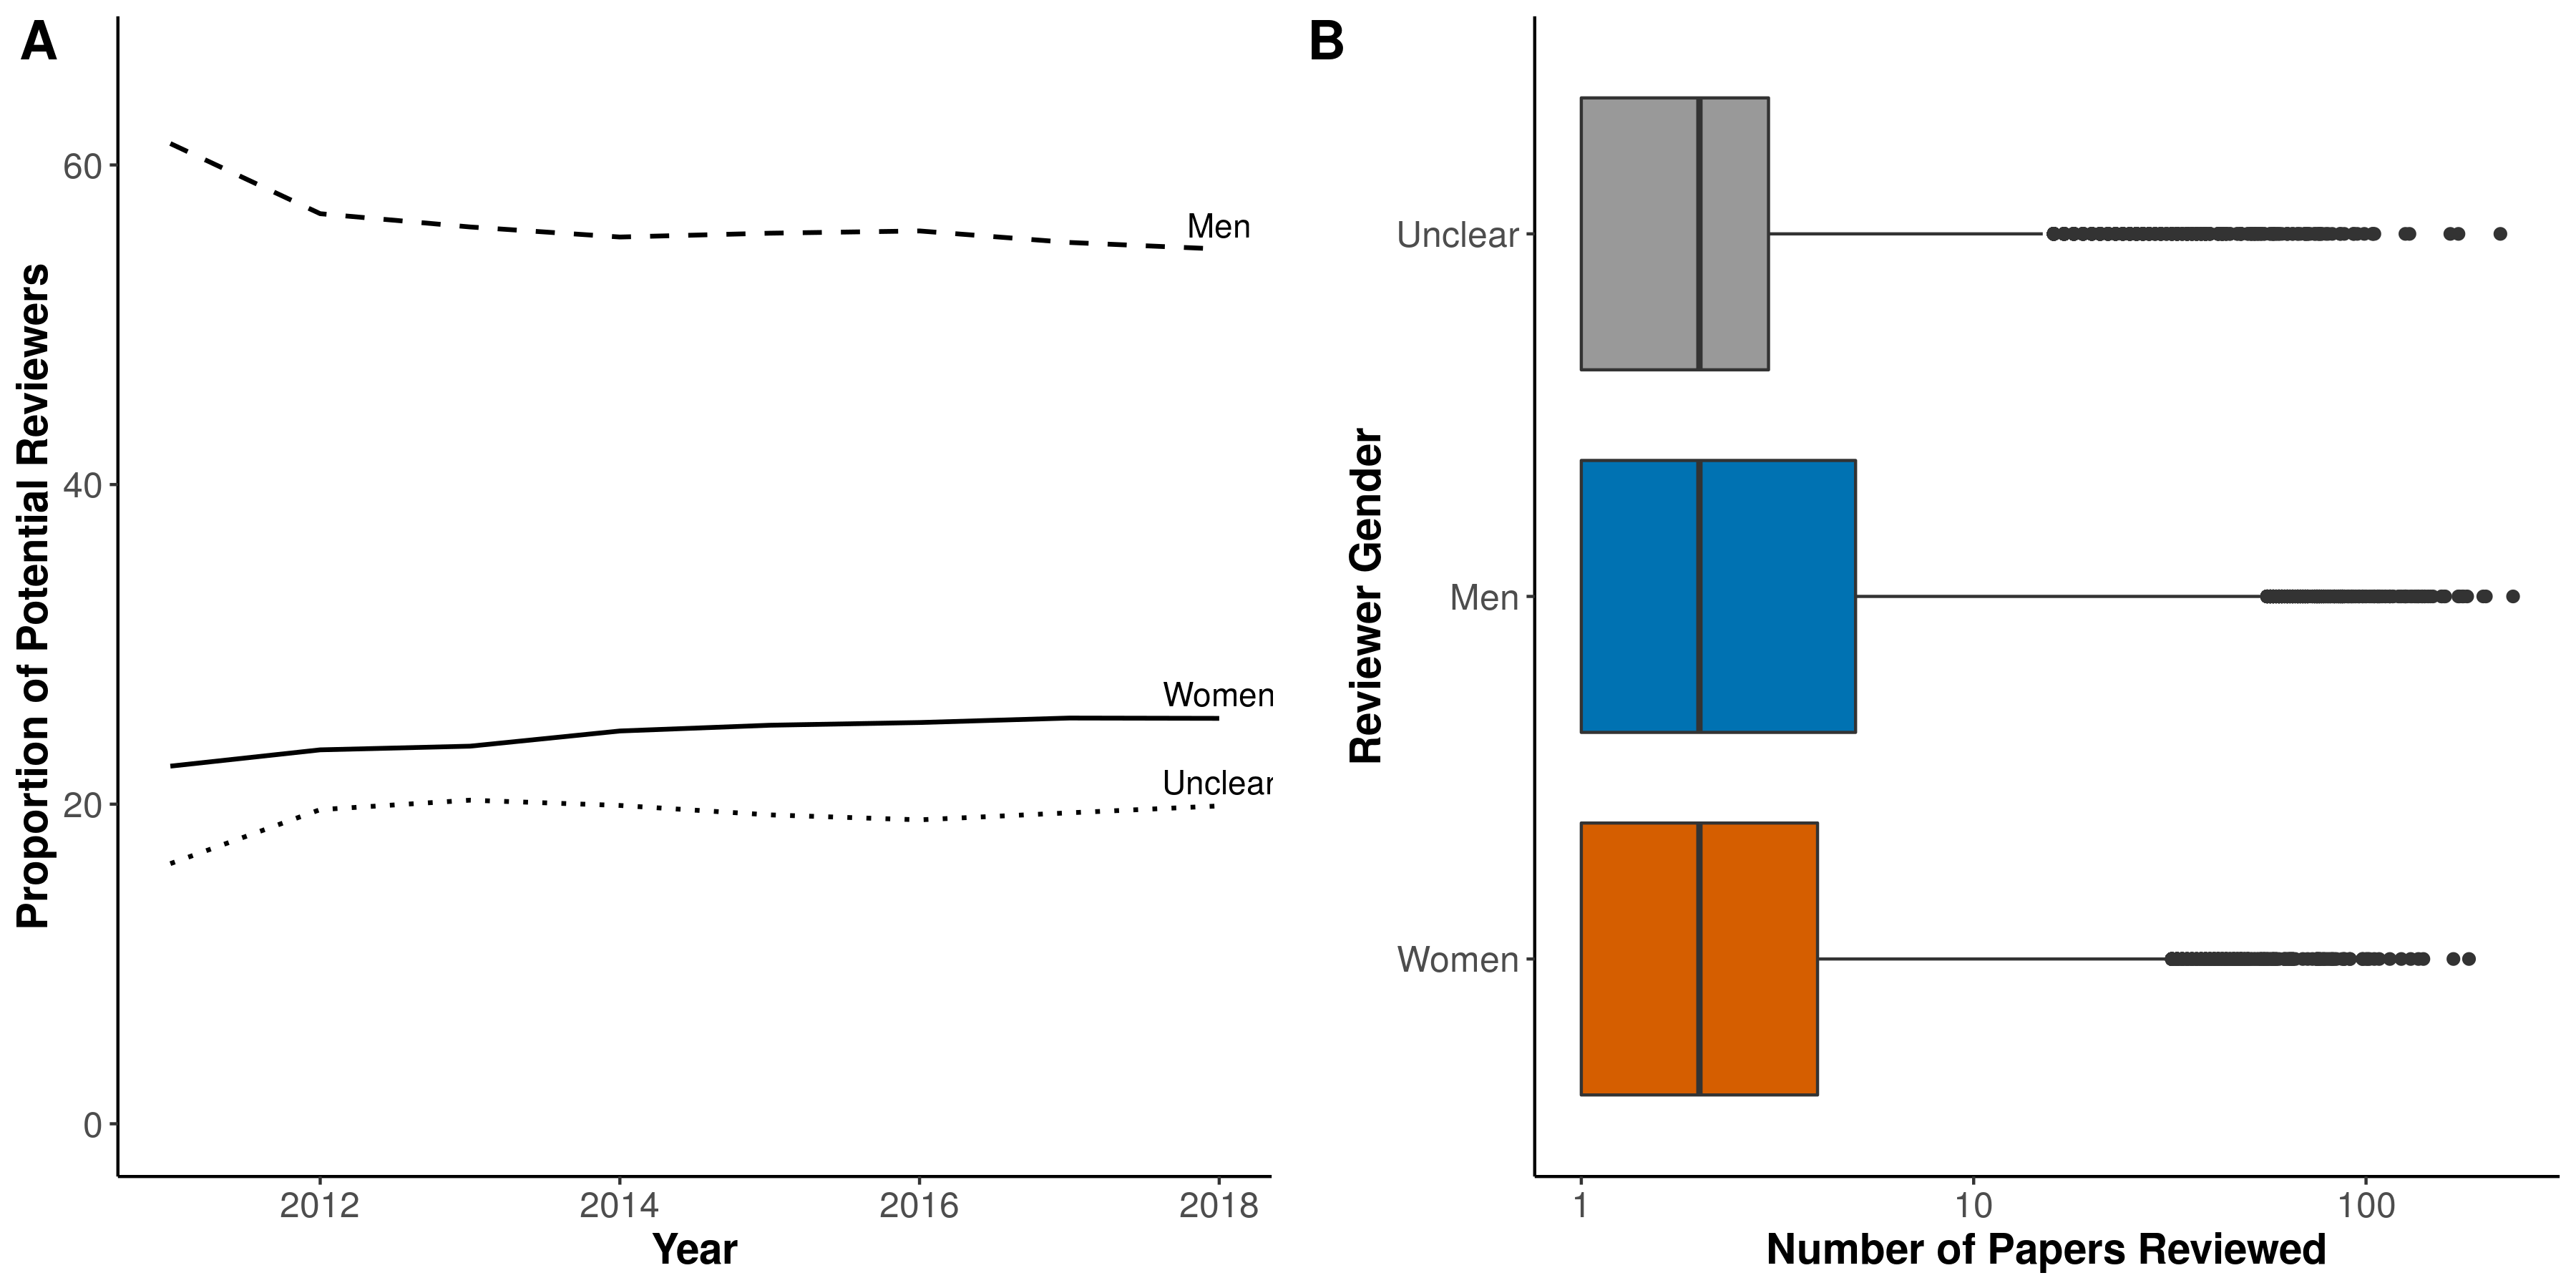
\includegraphics{Figure_2.png} \textbf{Figure 2. Reviewer
representation, workload, and response to requests to review.} (A)
Proportion of manuscript workloads by men and women editors. Editorial
rejections excluded. (B) Boxplot comparison of total papers reviewed by
each individual according to gender. (C) Percent of each reviewer gender
contacted to review, according to the editor's gender. (D) The percent
of reviewers by gender that either accepted the opportunity to review or
did not respond to a request to review, split according to the editor's
gender.

\textbf{Editorial workloads are not proportionate} Across all journals,
men handle a slightly greater proportion of manuscripts (blue) and women
a slightly smaller proportion (orange), relative to their respective
editorial representations (Fig. 1A). This trend continues accross most
journals with varying degrees of difference between workload and
representation (Fig. S1). There are exceptions. At \emph{mBio} and
\emph{mSphere}, workload and proportions are identical. However, at CVI
and JVI, the workload for women editors is much higher than their
representation, while the workload of men is considerably less than
their representation would suggest. In the years preceding its
retirement, the representation of women at CVI increased, which acted to
decrease the gap with their workload. However, representations and
relative workloads for men and women editors at JVI have held steady
over time.

The median number of papers reviewed by individuals in each gender group
is equivalent, with a trend to more men reviewing a greater quantity of
manuscripts (Fig. 2B). 3275, 6413, and 3176\% of men, women, and unknown
reviewers have reviewed only one manuscript. Editors of both genders
contact reviewers from all three gender groups at equivalent
proportions, though women editors contact more reviewers than men (Fig.
2C). Reviewers of all genders, accept fewer, and ignore more, requests
to review from women editors than men (Fig. 2D).

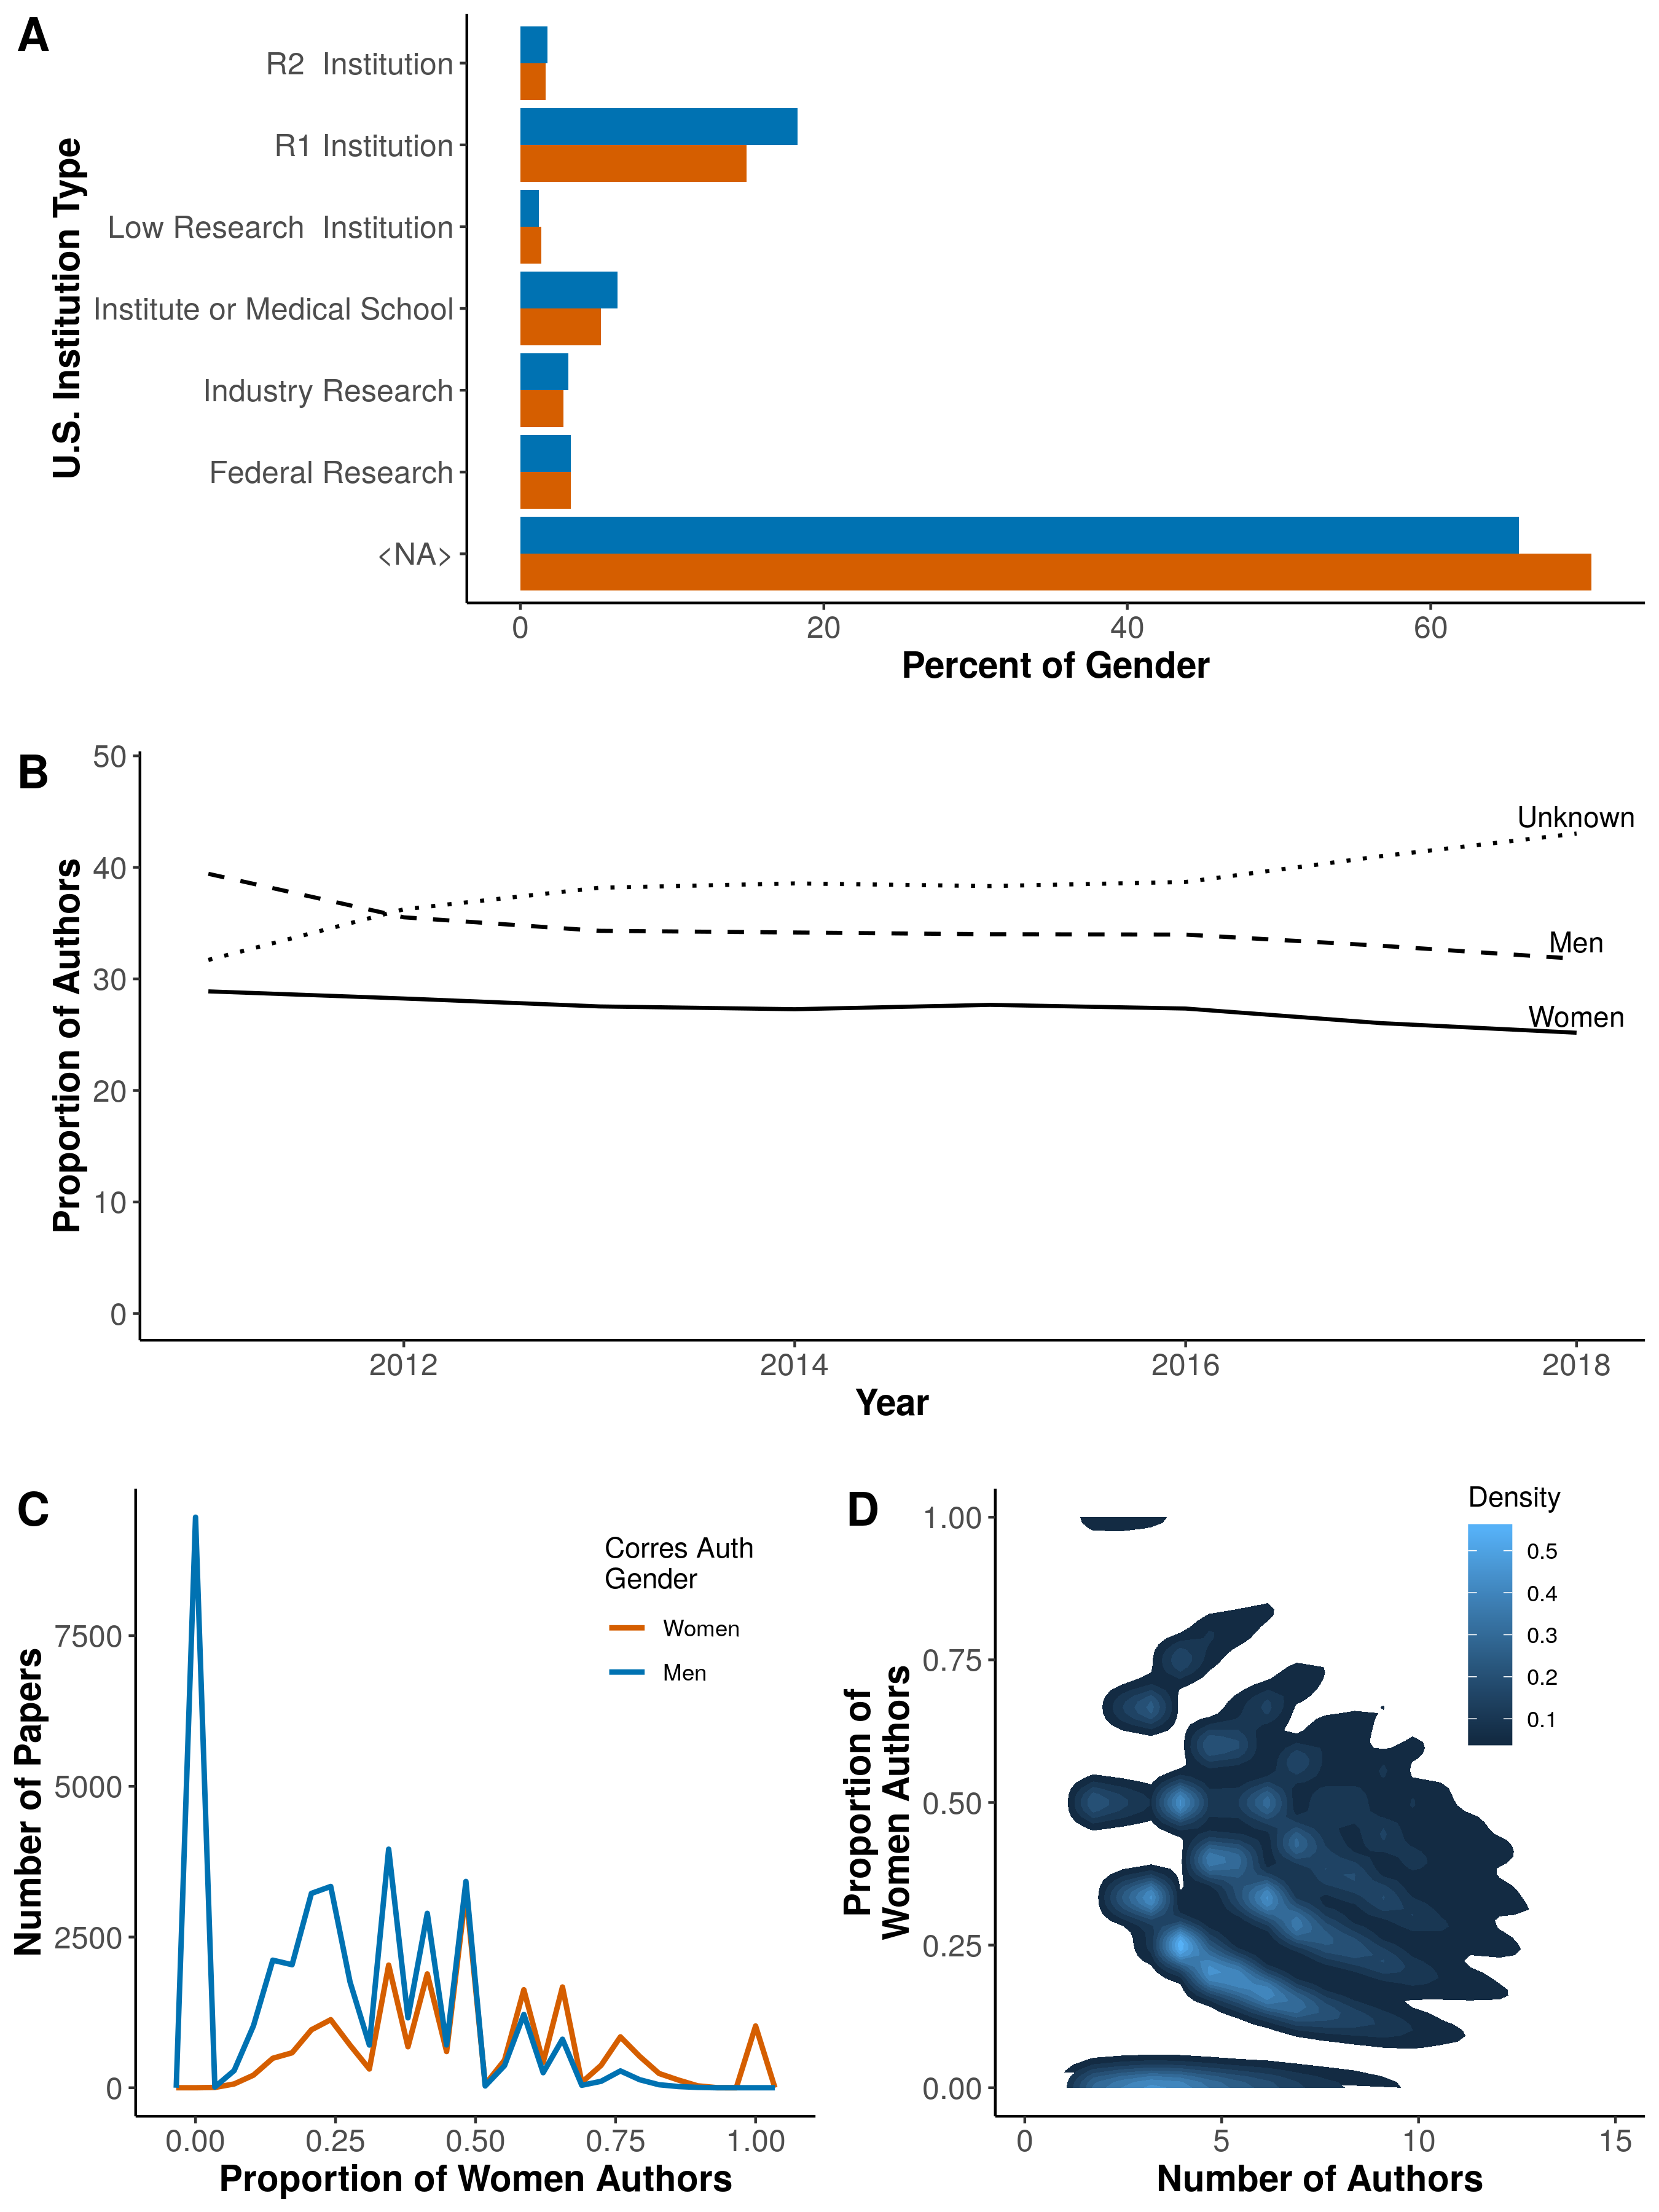
\includegraphics{Figure_3.png} \textbf{Figure 3. Author representation
by gender.} The proportion of (A) men and women authors from US
institutions, (B) men, women and unknown authors from 2012 - 2018.
Unique manuscripts submitted from 2012 to 2018. The proportion of (C)
first authors and (D) corresponding authors from 2012 - 2018. Solid
lines indicate individuals, dashed indicate proportion of manuscripts
submitted. Men indicated by blue and women by orange.

\textbf{Women are underrepresented as authors} The institution orgin of
submitting men and women authors is similar to that of editors and
reviewers, where over 60\% were from non-US institutions, followed by
20\% from R1 institutions (Fig. 3A). The proportions of men and women
authors at ASM have decreased over time at equivalent rates, with a
ratio of men to women authors of 4:3 since 2012 (or, 57\% men) (Fig.
3B). This decrease corresponds with an increase in the proportion of
unknown authors. Globally, microbiology researchers are 60\% men and
40\% women (Elsevier report). At ASM in September 2018, 38.37\% of
members who reported their gender, were women.

The proportion of papers submitted with men (blue dashed) and women
(orange dashed) first authors have remained constant with an average of
29.64 and 31.08 percent, respectively (Fig. 3C). Their respective
proportions of published manuscripts are nearly identical at 33.16\% for
men and 33.85\% for women. The proportion of submitted papers with men
corresponding authors has remained steady at an average of 42.45\% and
the proportion with women corresponding authors at 23.56\%. However,
their respective proportions of published manuscripts, 49.85\% for men
and 24.35\% for women, are dissimilar (Fig. 3D). The published
manuscript proportion where men are corresponding authors has a 7.4 gap
in percentage points, while the gap for women corresponding authors is
only 0.79. This trend is similar for middle and last authors (Fig.
S3AB).

To better visualize the 7.52 decrease in the proportion of women who are
first authors to those who are corresponding authors, we asked the
proportions at which women have been retained through the peer review
system at ASM journals.

There were 84482 men and 76215 women who were junior authors at ASM
journals during the period of time under study. Of those junior authors,
13.59 of the men were also senior authors, 16.72 considered as
reviewers, 11.11 actually reviewed, and 0.66 were editors at ASM
journals. At 8.25, 8.91, and 5.39, 0.25, just half as many women
progressed through each role at ASM journals.

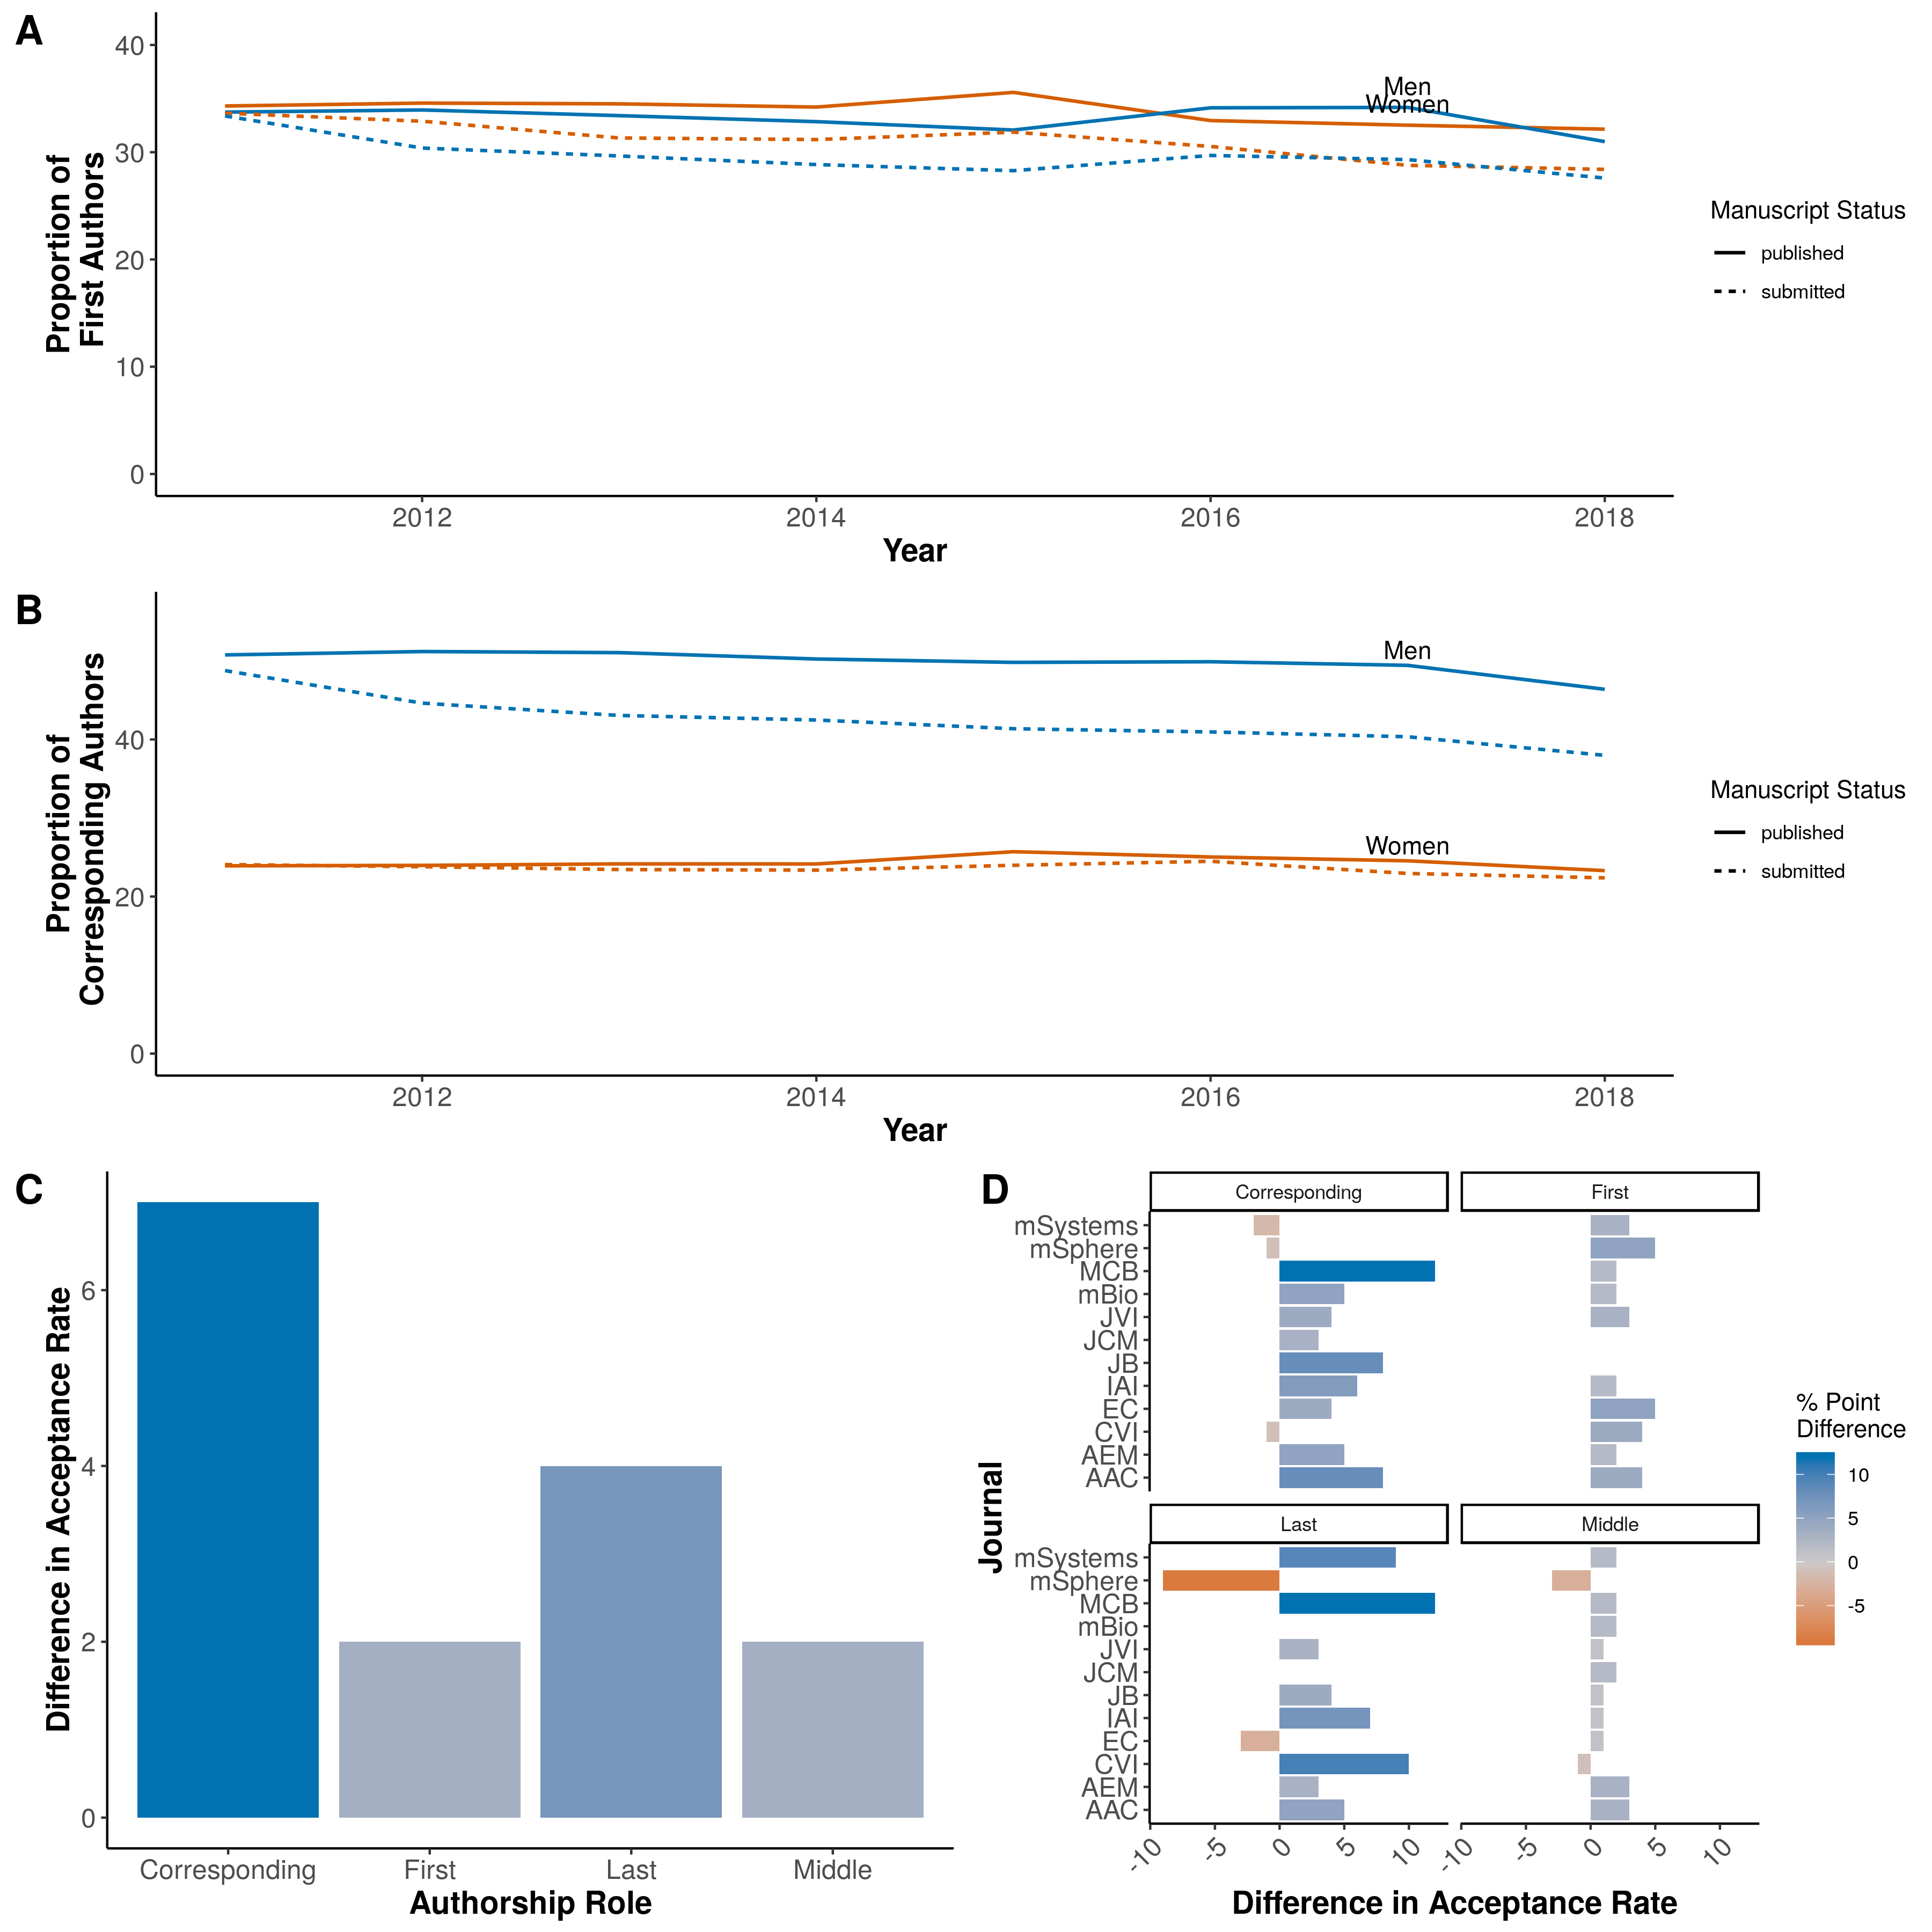
\includegraphics{Figure_4.png} \textbf{Figure 4. Difference in rejection
rates by corresponding author gender.} The percent of manuscripts
rejected by author gender and type (e.g., corresponding, first, last,
middle) at (A) all journals combined or at (B) each journal, which shows
the difference in percent rejection rates. (C) The difference in percent
editorial rejection rates at each journal, vertical line indicates the
difference for all journals combined. (D) The difference in percentage
points between each decision type following the first peer review,
vertical lines indicate the difference value for all journals combined.
The difference in rejection rates was determined by subtracting the
rejection rate of women-authored papers from men-authored papers within
each category. The shade (ranging from orange to blue) indicates the
outperforming gender. No bar indicates no difference in percentange
points.

\textbf{Papers submitted by women have more negative outcomes than those
submitted by men.} To better understand the percentage point difference
in gendered performance (Fig. 3D), we next compared the rejection rates
at each author stage. Middle authors were rejected at similar rates for
men and women, a 0.11 percentage point difference across all journals
combined. However, senior woman-authored manuscripts are rejected more
frequently than those authored by men with percentage point differences
of -2.26 and -1.2 for corresponding and last authors, respectively (Fig.
4A). Breaking it down by individual journals, there are several
instances where the overall trend is repeated or even amplified (e.g.,
AAC, IAI, JB, \emph{mBio}, MCB). The greatest effect was observed when
comparing the gender of corresponding authors, so we used this
sub-population to further examine the difference in acceptance/rejection
rates (Fig. 4A/S4).

We next compared the rejection rates for men and women corresponding
authors at two different bottlenecks, before and after the first peer
review. Papers authored by women are editorially rejected as much as 12
percentage points more often than those authored by men (Fig. 4B). The
percentage point difference at all ASM journals combined is -3.87
(vertical line), and two journals, MCB and \emph{mBio}, have more
extreme percentage point differences. Papers authored by men and women
are equally likely to be accepted after the first round of review (Fig.
4C, right panel). However, women-authored papers were rejected more
often (left panel) while men-authored papers were more often given
revision decisions (center panel). Three journals, JB, AAC, and MCB,
have percentage point differences more extreme than for all ASM journals
combined in both rejection (-5.5) and revision (5.46) decisions
(vertical lines).

In addition to manuscript decisions, other disparate outcomes may occur
during the peer review process. To determine whether women-authored
papers spent more time between being submitted and ready for
publication, we compared the number of revisions, days spent in the ASM
peer review system, and the number of days from submission to being
ready for publication to those authored by men. Papers authored by women
take slightly longer (from submission to ready for publication) than men
at some journals ( \emph{mSphere}, \emph{mBio}, \emph{mSystems}, CVI,
JB, JCM, AEM) despite spending similar amounts of time in the ASM
journal peer review system, and having equivalent median number of
revisions prior to acceptance (Fig. S5).

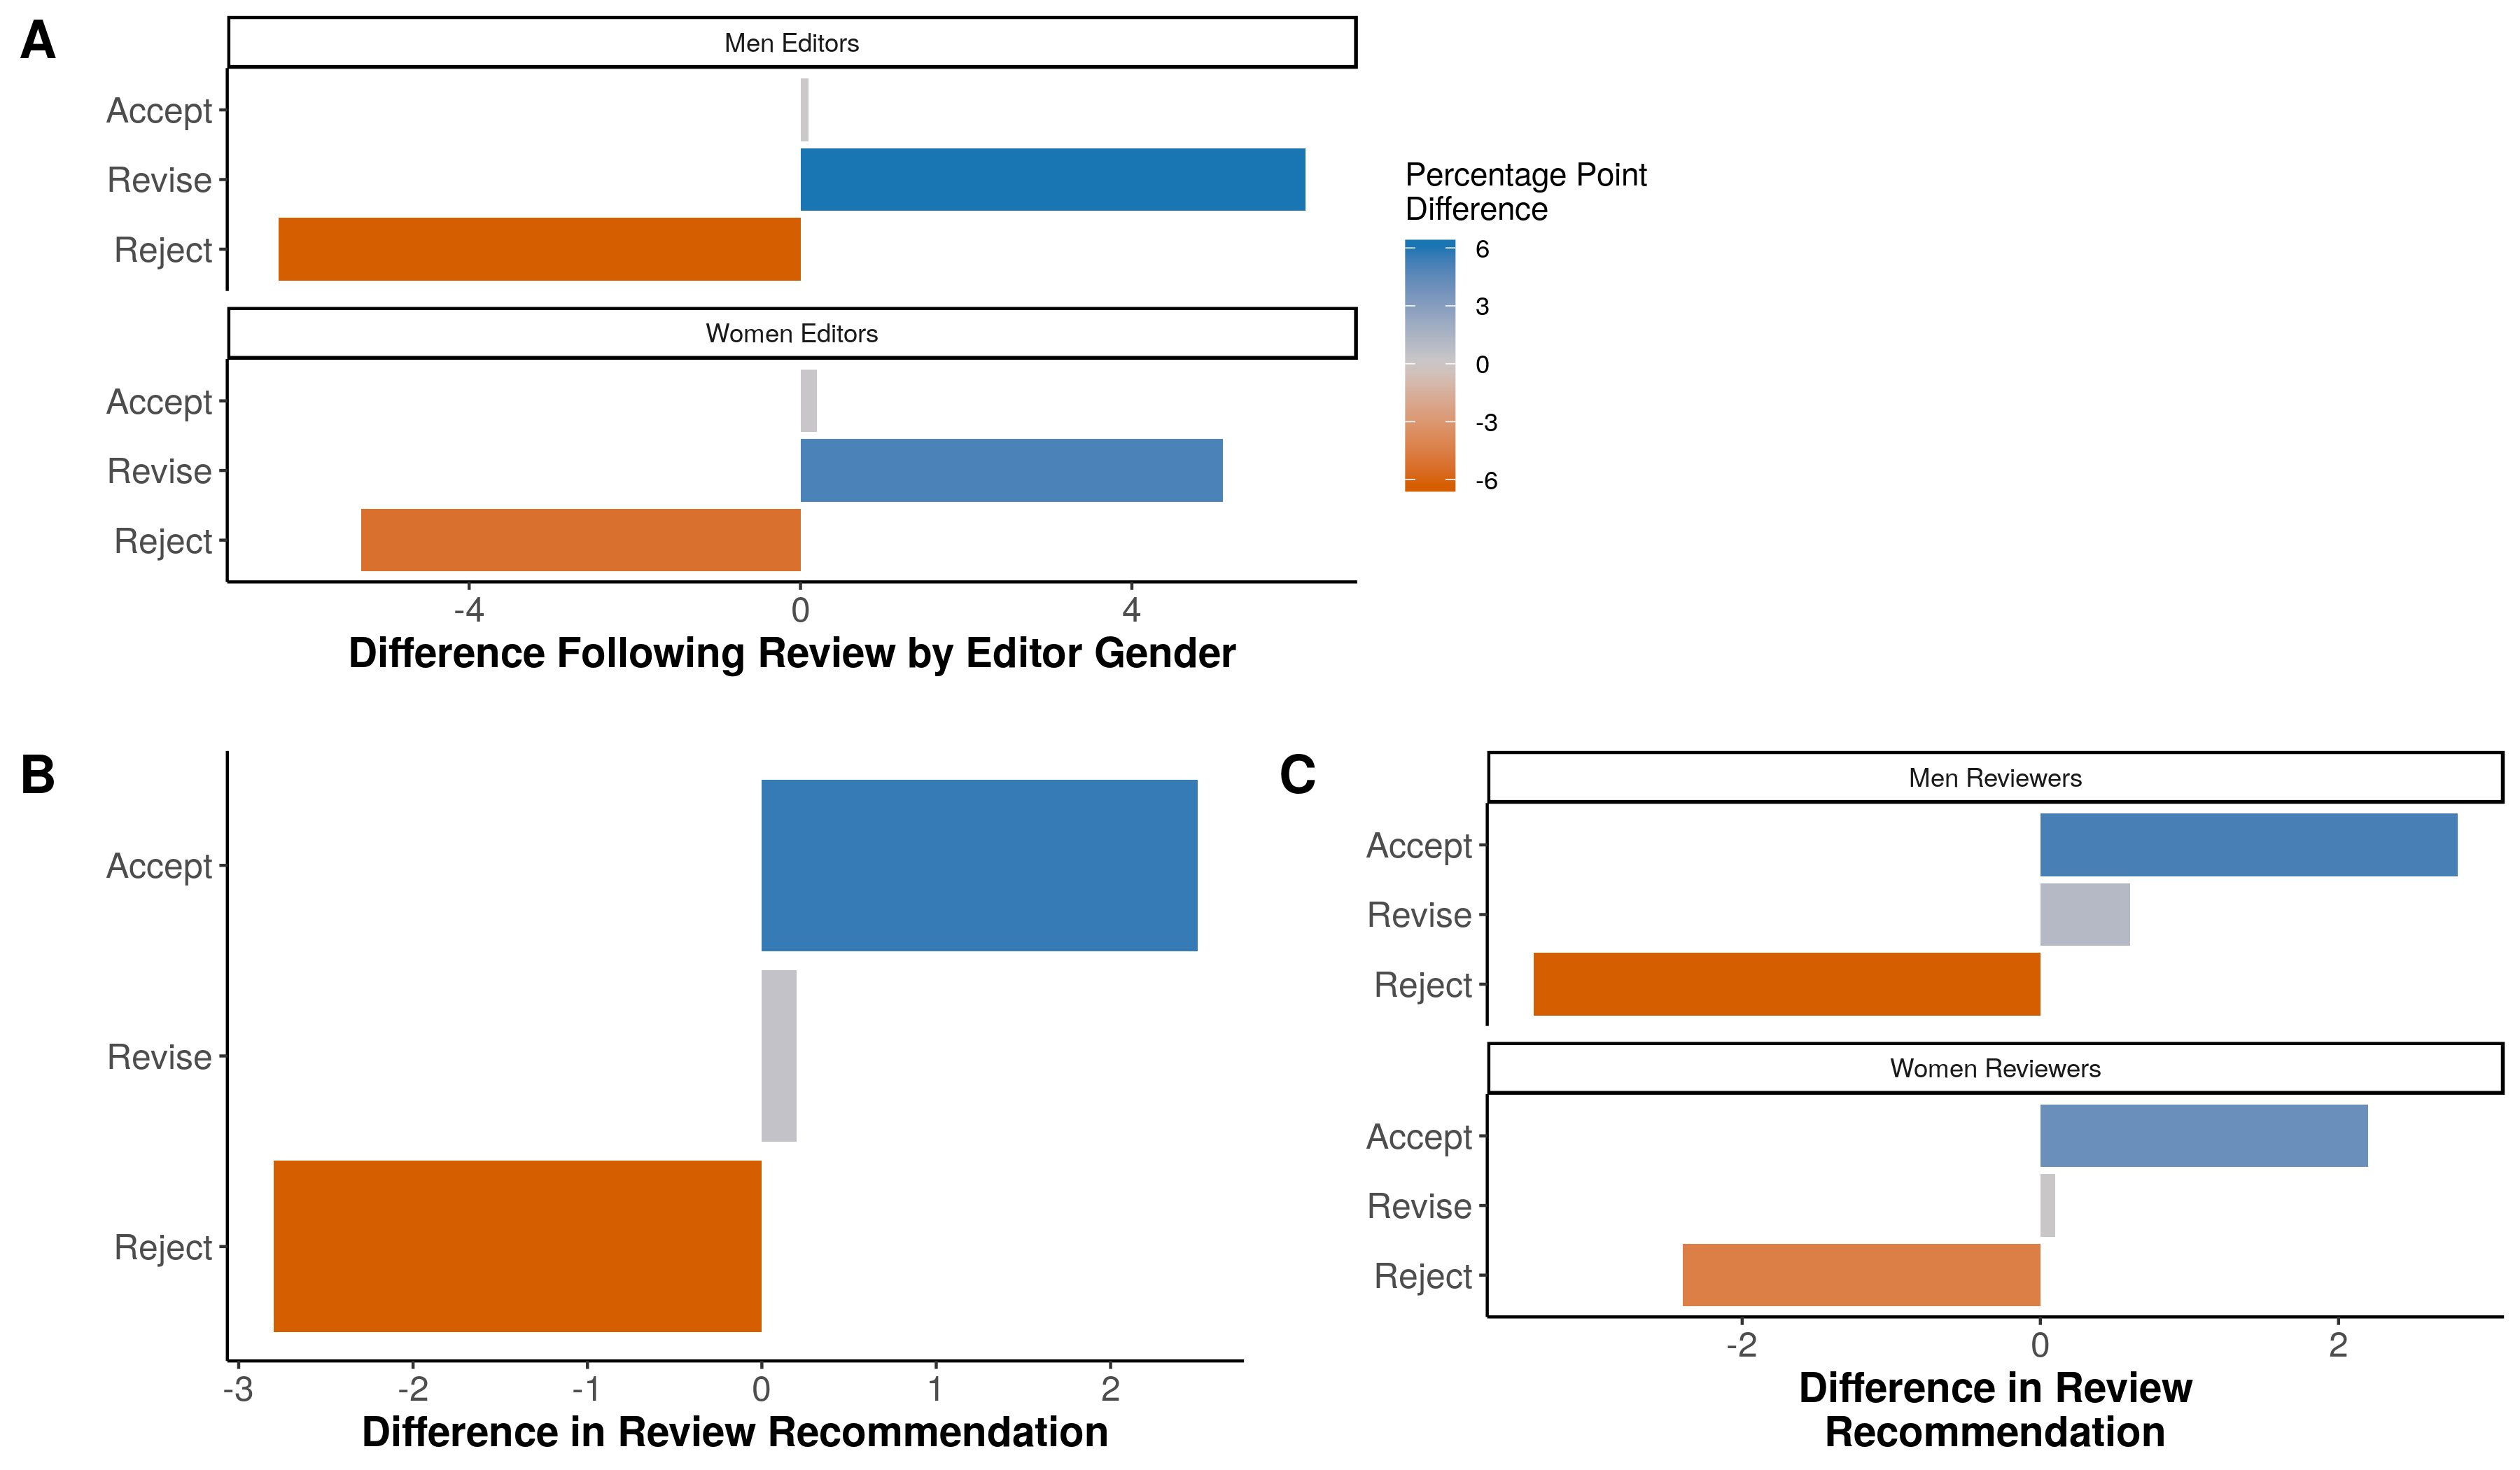
\includegraphics{Figure_5.png} \textbf{Figure 5. Difference in decisions
or recomendations according to the gatekeeper gender.} (A) Effect of
editor gender on the difference in percentage points for decisions
following review at all journals combined. (B) Difference in percentage
points for review recommendations and (C) how that is affected by
reviewer gender.

To understand how gatekeeper (editor/reviewer) genders influence
decisions (e.g., Fig. 4C), we grouped editor decisions and reviewer
suggestions according to the gatekeeper gender. Both men and women
editors rejected proportionally more women-authored papers, with men
editors making revise decisions on papers authored by men more often
than those authored by women (Fig. 5A). Reviewers are more likely to
suggest rejections for women as compared to men, though no difference in
revise suggestions were observed (Fig. 5B). Both men and women reviewers
recommended rejection more often for women-authored manuscripts though
only men reccomended acceptance more often for men-authored manuscripts
(Fig. 5C). Women reviewers suggested revision on women-authored papers
more often than men-authored manuscripts.

To evaluate whether or not manuscript decisions are random when gender
is taken into account, we used a logistic regression model to predict
whether or not a manuscript was reviewed (e.g., editorially rejected or
not). Our variables included the genders of the senior editor, editor,
and corresponding author, as well the proportion of authors that were
women. The median AUC of this model was 0.59, indicating that the
decisions are not completely random. However, because the value was
below 0.6 the included variables are not sufficent to create a reliable
model. This suggests that other factors influence gender-based
decisions.

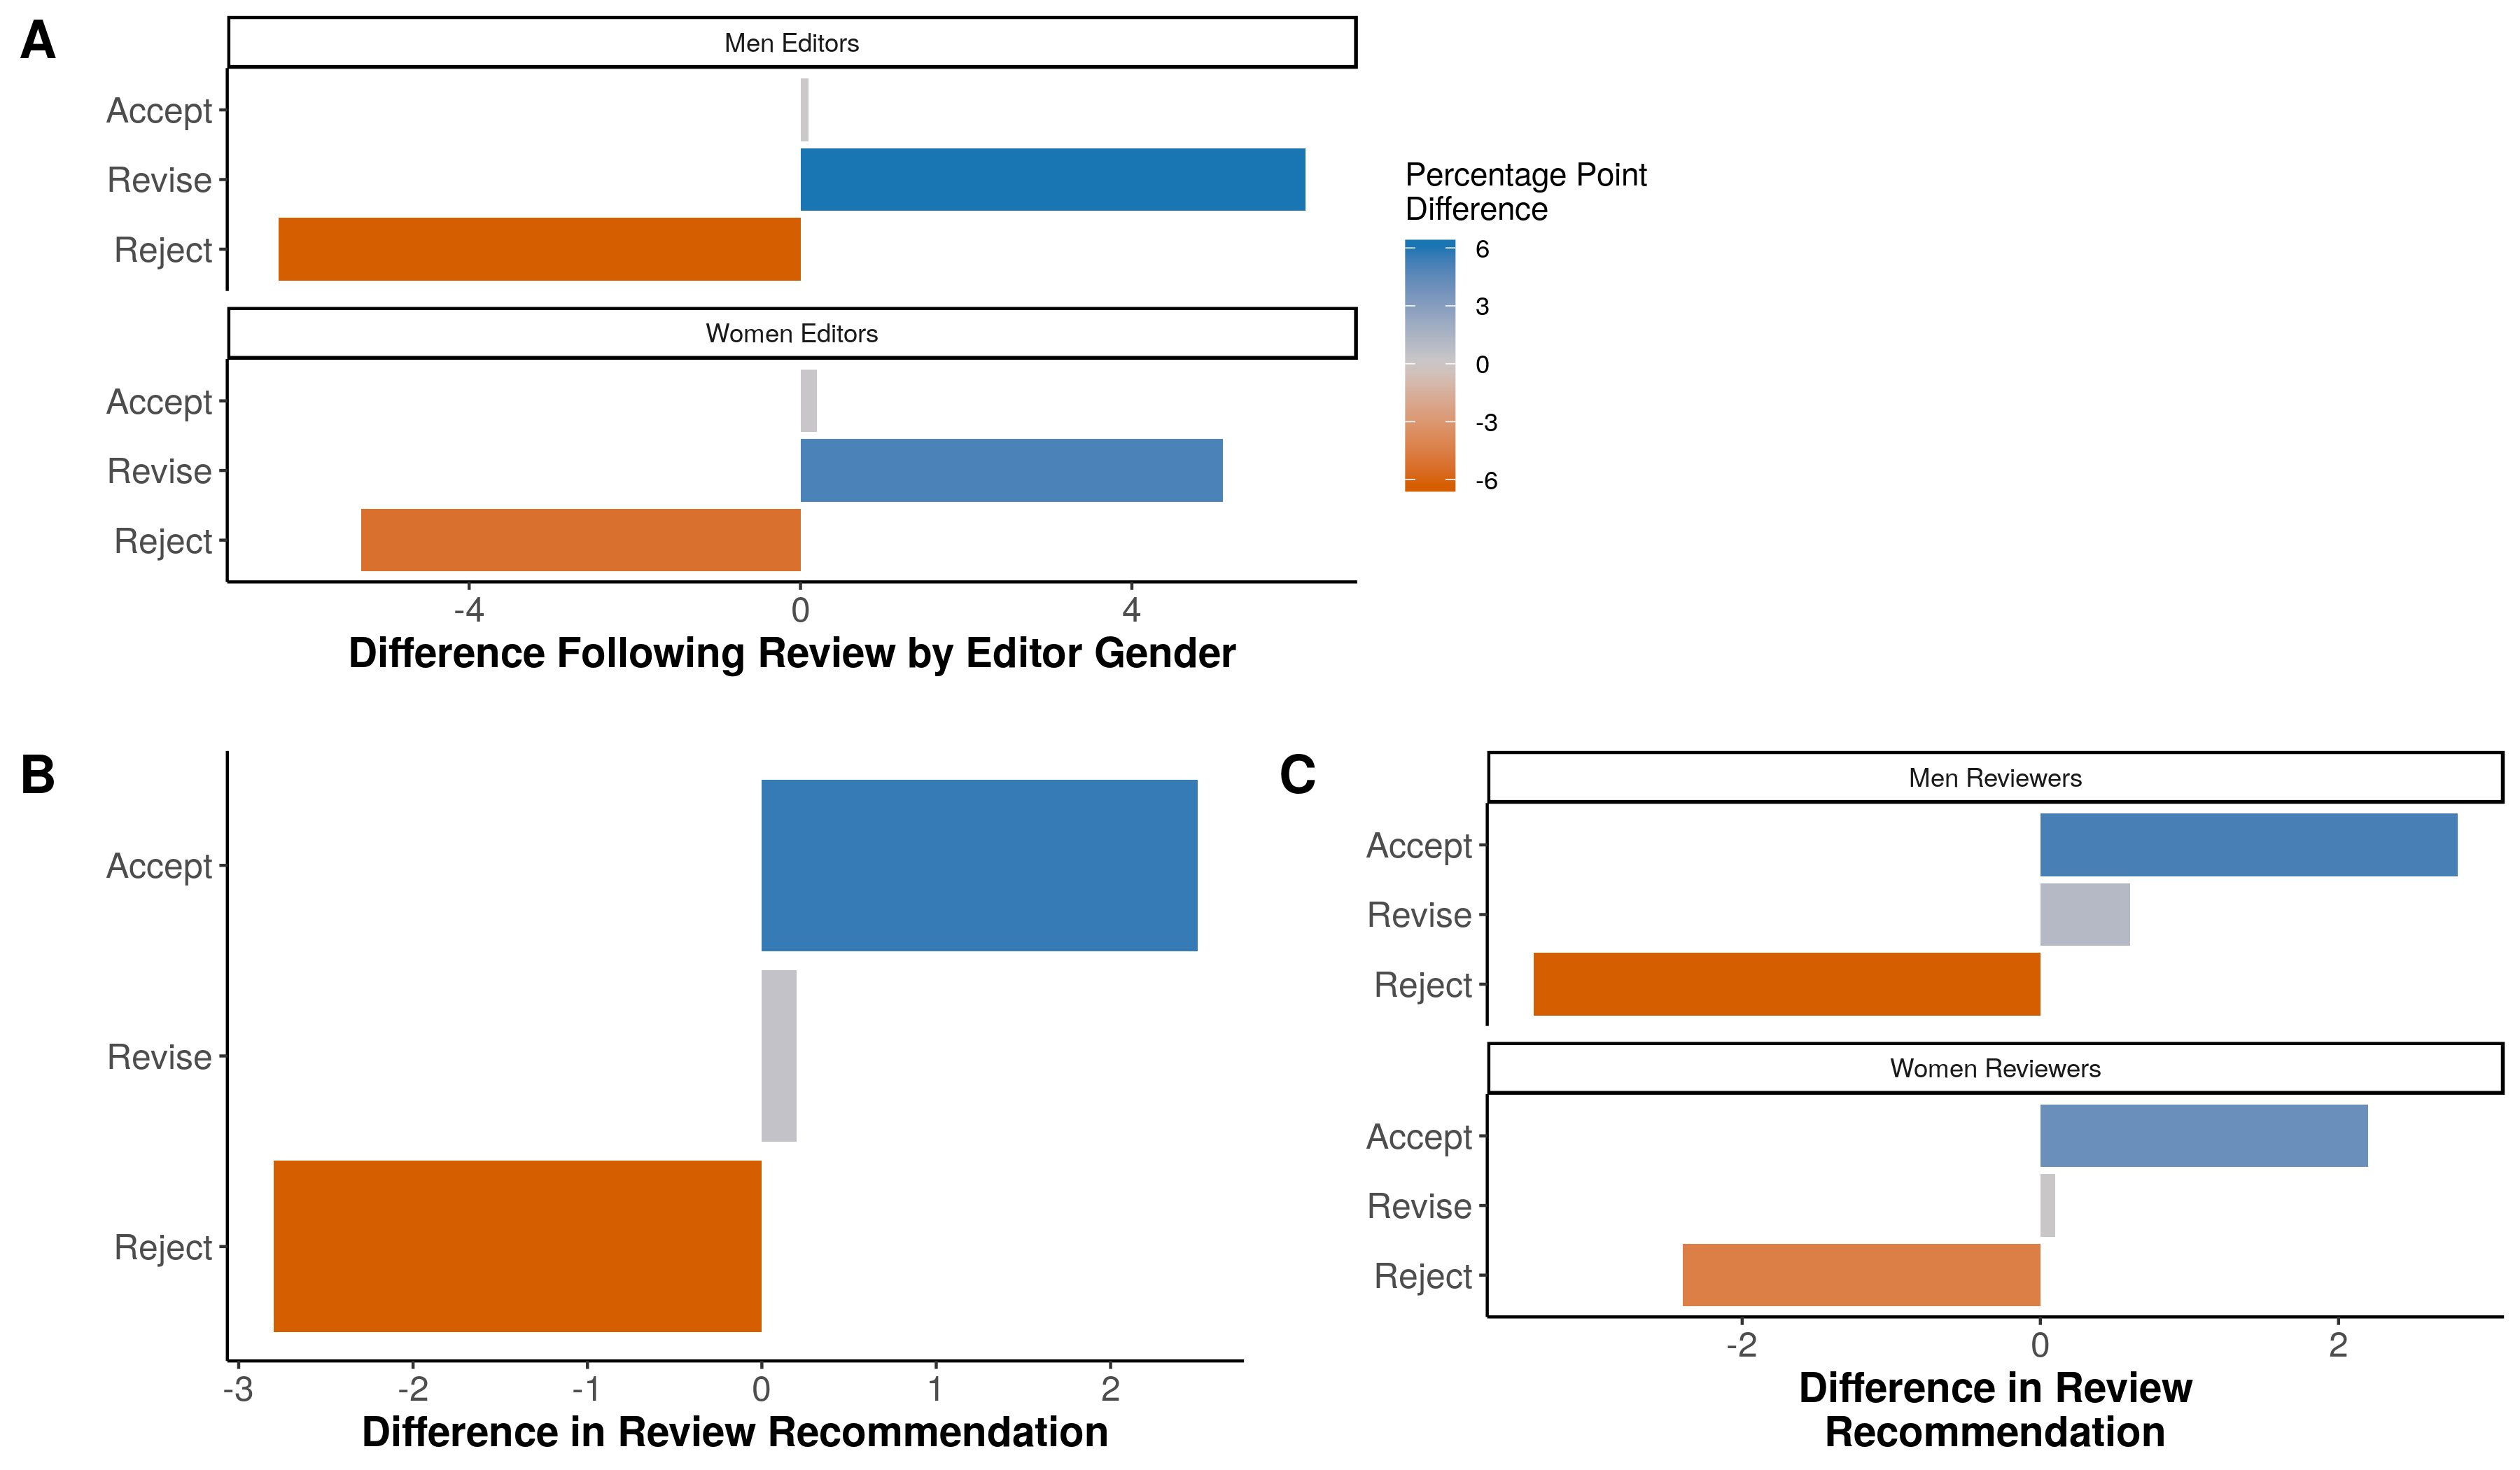
\includegraphics{Figure_6.png} \textbf{Figure 6. Impact of origin and
U.S. institution type on manuscript decisions by gender.} Difference in
percentage points for corresponding authors in the U.S. (A) editorial
rejections, (B) following first review, and by U.S. institution types
(C) acceptance and editorial rejections (D) acceptance decisions
according to editor gender. Vertical line indicates value for all ASM
journals combined. NA indicates non-categorized US institutions or
non-US institutions.

\textbf{Country and institute of origin contribute to overperformance by
men.} The issue of non-random, gender-based manuscript decisions could
be attributed to gender bias by journal gatekeepers, however, there are
other types of bias that may contribute to, or obsure, overt gender
bias. For instance, a recent evaluation of peer-review outcomes at
\emph{eLife} found evidence of geographic homophiliy, that is, reviewers
exhibited preference for research submitted by authors from their own
country or region (Murray, 2019). Other studies have documented prestige
bias, where men are overrepresented in more prestigous (i.e., more
respected and competent) programs (Weeden, 2017). It is therefore
possible, that what seems to be gender bias could be geographic or
prestige bias interacting with the increased proportion of women
submitting from outside the US or at lower prestige institutions (e.g.,
low research institutions) (Fig. 3A).

To try to separate how these factors affect manuscript decisions among
corresponding authors, we next looked at the outcome of papers submitted
only by corresponding authors at US institutions. When only considering
US-based authors, the difference in percentage points for editorial
rejections drops from -3.87 to -1.29, though trends across journals are
consistent (Fig. 6A). The difference in percentage points for decisions
after review mirror those of Figure 5, at the journal level (Fig. 6B).
There are also changes in the values for all journals combined. The
overperformance of women in rejection decisions decreases from -5.5 to
-3.47, and from 5.46 to 3.51, for the overperformance of men in revise
only decisions. The rate of accept decisions changed from -3.87 to -0.08
after restricting the analysis to US-based authors. These results
suggest that the country of origin (e.g, US versus not) accounts for
some gender bias, particulary for editorial rejections, but not all of
it.

To address prestige bias, we next split the US-based corresponding
authors according to their institution and re-evaluted the difference in
percentage points for men and women. Editorial rejections occured most
often for women from industry, R2, and medical schools or institutes
while manuscripts submitted by men from medical schools or institutes,
R1, and R2 instutitions were accepted more often than those submitted by
women (Fig. 6C). The occurence of rejections after review occured more
often for manuscripts submitted by women than those submitted by men,
regardless of editor gender (Fig. 6D). There are a couple of exceptions
where women authors from low research and industry research institutions
recieved more positive decisions by men editors. The institution types
from which manuscripts submitted by women had the greatest difference in
percentage points from those submitted by men are medical schools or
institutes and R2 institutions, with values of -20.37 and -6.28,
respectively.

To understand if these factors affect manuscript decisions in a
non-random manner, we used logistic regression model that took into
account both origin (US vs non), institution (US institution type) and
the genders of both gatekeepers and authors. This model predicted
whether or not a manuscript was published and had a median auc of 0.61
indicating non-random interaction between these factors. Those factors
with the greatest postive impacts on liklihood of publication were
X.inst.gender.Industry.Research.female.,
X.inst.gender.Industry.Research.male.,
X.inst.gender.Institute.or.Medical.School.male., US.inst.yes. The
factors with the greatest negative impacts on publication were
US.inst.no, X.inst.gender.R2..Institution.female.,
X.inst.gender.R2..Institution.male., inst.gender.NA.female. These
results confirm that the country of origin and prestige bias impact
decisions in a non-random manner, but gender-based factors are still at
play.

\subsection{Discussion}\label{discussion}

\begin{itemize}
\item
  summary of results
\item
  discuss representation
\item
  cite lit
\item
  interpret results

  \begin{itemize}
  \tightlist
  \item
    decreased response to F editors may increased editorial burden for
    men?
  \item
    does fewer collaborations contributed to decreased retainment
  \item
    remember to hammer trends \& diversity of journals
  \end{itemize}
\item
  why does it matter?
\end{itemize}

The under representation of women as corresponding authors in
publication at ASM journals has negative consequences for their careers
and microbiology. Buckley et al, suggest that being selected as a
reviewer increases visibility of a researcher, which has a direct \&
significant impact on salary. Therefore, the underrepresentation of
women as reviewers hampers their career progression and even their
desire to progress since reviewing also signals adoption of the
researcher into the scientific community (Buckley et al, 2014). This is
supported by Lerback and Hanson who noted that ``It {[}reviewing{]}
provides positive feedback that a scholar is respected and participating
in their field and fosters self-confidence, all of which lead to
increased retention of women.'' (Lerback \& Hanson, 2017) Retention of
women in science is important to the progress of microbiology as a field
since less diversity in researchers limits the diversity of
perspectives, approaches, and thus stunts the search for knowledge. In
addition to boosting productivity and knowledge, more diverse and
equitable organizations are more inclusive and supportive for all
members (Potvin, 2018). It is thus a moral and scientific imperity for
scientific societies and journals, such as ASM, to improve its own
diversity, equity and inclusion efforts. The remainder of this
manuscript will focus on actions that can be taken at multiple levels of
the peer review system to support these efforts.

\begin{itemize}
\tightlist
\item
  Discuss acceptance/rejection rates

  \begin{itemize}
  \tightlist
  \item
    submission vs decision question of representation
  \item
    W asked to do more work by reviewers? (increased rej + increased
    time + same vers)
  \item
    cites
  \item
    why it matters, compare
  \end{itemize}
\end{itemize}

Addressing bias (gender, geographic, prestige or otherwise) during peer
review process is a more difficult challenge, since it is partially the
result of accumulated disadvangates and microaggressions (the actions
resulting from implict biases). Implict bias training for gatekeepers is
a start, as might be double-blinded peer review, a common practice in
social sciences. To support efforts of making peer review more
transparent, the review process could be unblinded following the
editor's final decision on a manuscript. However, these solutions are
only bandaids on a deeply infected wound, since both focus on the
superficial issue of individuals instead of the underlying structure of
the system that has selected for the bias at hand.

Few papers have found disparities between rejection rates of men and
women and to our knowledge, this is the first paper to collectively
examine this issue with either submissions data from 10+ journals or on
the field of microbiology. Critics might argue that the effect size is
too small to really matter or that there are too many unaccounted
factors to draw conclusions. We acknowledge that these are limitations
of our study along with a limited journal dataset, an absence of
reviewer comments for sentiment analysis, and that many ASM journals
have a narrow focus while the broad scope journals are relatively new.
All of these factors prevent us from generalizing our results across
microbiology as a field. However, the consistency of the trends to
benefit men corresponding authors over women, across all journals
included and literature to-date confirms that this study is highly
relevant for the ASM as a society and offers opportunities to address
both gendered representation in microbiology and systemic barriers to
peer review at our journals. + descriptive papers don't have confounding
factors!

\subsection{Data and Methods}\label{data-and-methods}

\textbf{Data} All manuscripts handled by ASM journals (e.g.,
\emph{mBio}, \emph{Journal of Virology}) that received an editorial
decision between January 1st, 2012 and August 31st, 2018 were supplied
as XML files by ASM's publishing platform, eJP. Data were extracted from
the XML documents provided using R statistical software (version 3.4.4)
and the \texttt{XML} package (R citation). Data manipulation was handled
using the \texttt{tidyverse}, \texttt{lubridate}, and \texttt{xml2}
packages for R. Variables of interest included: the manuscript number
assigned to each submission, manuscript type (e.g., full length
research, erratum, editorial), category (e.g., microbial ecology),
related (previously submitted) manuscripts, versions submitted, dates
(e.g., submission, decision), author data (e.g., first, last, and
corresponding authorship, total number of authors), reviewer data (e.g.,
reviewer score, recommendation, editor decision), and person data
(names, institutions, country) of the editors, authors, and reviewers.
For this analysis, only original, research-based manuscripts were
included, e.g., long- and short-form research articles, New-Data
Letters, Observations, Opinion/Hypothesis articles, and Fast-Track
Communications.

Data were visualized using the ggplot, scales, RColorBrewer, and
ggalluvial packages for R.

\textbf{Defining manuscript outcomes} Many papers are immediately
rejected by editors/EICs instead of being sent to peer review, often due
to issues of scope or percieved quality. These were defined as editorial
rejections and identified as manuscripts rejected without record of
review. Alternately, editors could send papers out for review by two or
three experts in the field. The reviewers make suggestions to the editor
who decides whether the manuscript in question should be accepted,
rejected, or sent back for revision. At ASM journals, manuscripts with
suggested revisions that are expected to take more than 30 days are
rejected, but generally encouraged to resubmit. If resubmitted, the
authors are asked to note the previous (related) manuscript and the
resubmission is assigned a new manuscript number. Multiple related
manuscripts were tracked together by generating a unique grouped
manuscript number based on the recorded related manuscript numbers. This
grouped manuscript number served multiple purposes including: tracking a
single manuscript through multiple rejections or transfers between ASM
journals and to avoid duplicate counts of the same authors for the same
manuscript.

\textbf{Institution classification} To identify the communities
represented, we used Carnegie classifications to group US-based
insititutions into R1, R2, low (not R1 or R2), and medical research.
Medical schools and institutions (e.g., Mayo clinic) were grouped
together. Two other categories were added to represent industry and
federal research. The other category represents uncategorized US
institutions.

\textbf{Bias analysis and presentation} To identify potential biases, we
calculated the difference in percentage points between a given outcome
for men and women, e.g., the percentage point difference in acceptance
rates is the acceptance rate for men minus the acceptance rate for
women. A positive value indicates that men receive the outcome more
often than women, whereas a negative value indicates that women
outperform men in the given metric. To correct for the disparity in the
participation of women relative to men at ASM journals, all percentage
point comparisions are made relative to the gender and population in
question.

\textbf{Logistic regression models} For the L2-regularized logistic
regression models, we established modeling pipelines for a binary
prediction task. First, we randomly split the data into training and
test sets so that the training set consisted of 80\% of the full dataset
while the test set was composed of the remaining 20\% of the data. To
maintain the distribution of the 2 model outcomes that was found with
the full dataset, we performed stratified splits. The training data was
used to build the models and the test set was used for evaluating
predictive performance. To build the models, we performed an internal
five-fold cross-validation where we tuned the \textbf{cost}
hyperparameter which determines the regularization strength where
smaller values specify stronger regularization. This internal
cross-validation was repeated 100 times. Then, we trained the full
training dataset with the selected hyperparameter values and applied the
model to the held-out data to evaluate the testing predictive
performance of each model. The data-split, hyperparameter selection,
training and testing steps were repeated 100 times to get a reliable and
robust reading of model performance. Models were trained using the
machine learning wrapper caret package (v.6.0.81) in R (v.3.5.0).

\textbf{Gender prediction and assignment} The gender assignment API
genderize.io was used to predict an individual's gender based on their
given names, and country where possible. The genderize.io platform uses
data gathered from social media to predict gender based on given names
with the option to include an associated language or country to enhance
the odds of successful prediction. Since all manuscripts are submitted
in English, precluding language association for names with special
characters, names were standardized to ASCII coding (e.g., ``José'' to
``Jose''). We next matched each individuals country against the list of
X country names accepted by genderize.io. Using the
\texttt{GenderGuesser} package for R, all unique given names associated
with an accepted country were submitted to the genderize.io API and any
names returned without a predictive assignment of either male or female
were resubmitted without an associated country. All predictive
assignments of either male or female are returned with a probability
match of 0.50 or greater. The predicted genders of all given names (with
and without an associated country) whose probabilities were greater or
equal to our arbitrary success cut off of 0.65 were used to assign
predicted gender to the individuals in our dataset. Predicted genders
were assigned to individuals in the following order: first names and
country, first names, middle names and country, middle names (Fig. S7).
The presenting gender (man/woman) of editors and senior editors in our
dataset was hand validated using Google where possible.

We recognize that biological sex (male/female) is not always equivalent
to the gender that an individual presents as (man/woman), which is also
distinct from the gender(s) that an individual may self-identify as. For
the purposes of this manuscript, we choose to focus on the presenting
gender (man/woman/unknown) based on their first names and/or appearance
(for editors). In the interest of transparency, we include those
individuals whose names don't allow a high degree of confidence for
gender assignment in the ``unknown'' category of our analysis.

\textbf{Validation of gender prediction} We first validated the
algorithm using a set of 3265 names whose gender had been hand-coded
based on appearance and were generously provided to us by \_\_\_
(preprint cite). The names were supplied to the genderize algorithm both
with and without the accompanying country data. The data returned
include the name, predicted gender (male, female, na), the probability
of correct gender assignment (ranging from 0.5 to 1.0), and the number
of instances the name and gender were associated together (1 or
greater). The genderize algorithm returned gender predictions for 2899
when first names were given and 2167 when country data was also supplied
(732 names were associated with countries unsupported by genderize).

Sensitivity and specificity, are measurements of the algorithm's
tendency to return correct answers instead of false positives (e.g., a
man incorrectly gendered as a woman) or false negatives (e.g., a woman
incorrectly gendered as a man). The closer these values are to 1, the
smaller the chance that the algorithm will return the correlating false
response. Accuracy is a composite measure of the algorithm's ability to
differentiate the genders correctly. These measurements were calculated
from the datasets (with and without country data supplied) at three
different probability threshold cutoffs: the default genderize (0.5), a
probability threshold of 0.85 (0.85), and a modified probability of
0.85, which factors in the number of instances returned
(pmod0.85)(citations).

At the 0.5 threshold, the dataset returned a sensitivity of 0.8943 and
specificity of 0.9339 for an accuracy of 0.911, compared to a marginally
higher accuracy of 0.9146 for the dataset where country data were
included (Table S1). Generally speaking, the accuracy increases as the
threshold increases along with slight trade offs between sensitivity and
specificity. For the purposes of our analysis, we opted to use the
pmod0.85 threshold moving forward (Table S1, in bold).

To understand the extent of geographic bias in our gender assignment
against regions and languages with genderless naming conventions, or
that lack social media for incorporation into the genderize algorithm,
we compared the number of names predicted without associated country
data to when country data was also supplied. In our test dataset, the
top five countries associated with names were United States, Germany,
United Kingdom, France, and China and the countries with the highest
proportion of un-predicted genders when country data were supplied are
Cambodia, Iceland, Indonesia, Ireland, and Mexico, where the maximum
number of names supplied ranged from 1 to 15. To determine the impact of
each country towards the overall percentage of names whose genders were
not predicted (27.14\%), we found the difference between the percent of
names unpredicted for each country and the overall percentage,
multiplied by the proportion of observations from that country to the
total observations and finally divided by the overall percentage of
unpredicted names (Fig. S8). The top five countries with the greatest
impact on unpredicted names, and thus the countries receiving the most
negative bias from genderize were Canada, China, Ireland, Belgium, and
Sweden (Fig. S9). These data suggest that there is likely some bias
against countries with gender-neutral naming conventions (China), and
indicates the stringency with which the algorithm applies gender to
names that are accompanied by country data. For instance, strongly
gendered names such as Peter and Pedro were not assigned gender when
associated with Canada.

We next applied the genderize algorithm at the pmod0.85 threshold to our
journals dataset and tested its validity on a small portion. All first
names collected from our dataset were submitted to genderize both with
and without country data. Only those predictions whose pmod were
equivalent or greater than 0.85 were carried to the next step. The
predicted genders were assigned to individuals in the following order:
first names and country, first names, middle names and country, middle
names. Given the relatively small number of editors and senior editors
in our dataset, the presenting gender (man/woman) of editors and senior
editors in our dataset was hand-validated using Google where possible.
Of the 1072 editor names, 938 were predicted by genderize for an
accuracy of 0.9989339, thus increasing our confidence in the gender
predictions where made.

In our full dataset, the five countries with the most individuals were
United States, China, Japan, France, and Germany and the countries with
the highest proportion of un-predicted genders were Burundi, Chad,
Kingman Reef, Korea (North), Democratic People's Republic of, and
Maldives, where the maximum number of names supplied ranged from 1 to 4.
Proportionally, fewer names in our full dataset were assigned gender
than in our validation dataset (40.01\% unpredicted versus 27.14\%
unpredicted, respectively). Since adjusting the workflow to predict the
gender of names both with and without country data, the countries
receiving the most negative bias from genderize were China, Japan,
Korea, Republic of, India, Taiwan, Province of China (Fig. S10). These
data indicate what we previously predicted, that the genderize algorithm
has bias against countries with gender-neutral naming conventions.

\textbf{Code availability} The code for all analysis steps, logistic
regression pipeline, and an Rmarkdown version of this manuscript, is
available at \url{https://github.com/SchlossLab/Hagan_Gender_mBio_2019/}

\textbf{Acknowledgements} We would like to thank Nicole Broderick and
Arturo Casadevall for providing their dataset for genderize validation
and acknowledge Arianna Miles-Jay and Joshua MA Stough for their
comments.

A.K.H. was responsible for project and experiment design, data analysis,
and drafting the manuscript. B.T. completed the logistical regression
models. P.S. provided funding, resources and conceptual advice. All
authors contributed to the final manuscript. P.S. is Chair of ASM
Journals and A.K.H. was ASM staff prior to publication of the analysis.
B.T. reports no conflict of interest.

Funding for this work was provided by the American Society for
Microbiology. The sponsors had no role in study design or
interpretation.

\subsection{References}\label{references}


\end{document}
